\section{Network of ``Parameterization Prediction"}
In this section, we first explain the general structure of our proposed network, and then in Sec~\ref{subsec:k-n_point_net}\ref{subsec:conv}\ref{subsec:deconv} we explain the details of its structure. In Sec~\ref{subsec:variation}, we explain a few variation of the network design that we have explored.
\subsection{Network Overview}
\begin{figure}[htbp]
	\centering
	\includegraphics[width=\linewidth]{img/net/overview}
	\caption{The overview of the network: The parameterization network is built by stacking k-neigbor point net blocks (with $k=16,12,10,8$ in the picture). It predicts point-wise offset and add then to input point set. The semantic network is built by convolution and deconvolution networks. It takes image and a random vector as input to predict parameters for the parameterization network}
	\label{fig:overview}
\end{figure}
Our basic idea is to use convolution and deconvolution network that takes image as input to predict parameters for the parameterization network that deform/map a point set uniformly sampled from the surface of a unit sphere to the target point set. Figure~\ref{fig:overview} illustrates the overview of our network. The parameterization network is built by stacking several K-neighbor PointNet (explained in Sec~\ref{subsec:k-n_point_net}). Each k-neighbor point net predicts a point-wise offsets and add them to the sampled points. In this way, the parameterization network can map a randomly sampled point set to target shape. By using different randomly generated samples from the parameter domain in the training and testing, the parameterization network can simulate the \textit{sampling variation} that is introduced by using specific point set as ground truth. The semantic network is built by convolution and deconvolution layers, it takes normally distributed random vector and a input image as input to predict the parameter for the parameterization network. In this way, the semantic network relates the input image to the shape manipulation and uses normally distributed random vector to encode the \textit{semantic variation} that is introduced in the irreversible 3D-to-2D projection. The entire network is built by differentiable operations, making it end-to-end trainable.
\subsection{K-neighbor Point Net for Parameterization Network} 
\label{subsec:k-n_point_net}
\begin{figure}[htbp]
	\centering
	\includegraphics[width=\linewidth]{img/net/k-n_pointnet}
	\caption{The structure of K-neighbor Point Net: Orange boxes indicate operations/layers. Light blue boxes indicate tensors. The green boxes indicate predicted parameters ( i.e. output of semantic network ). All the MLP have only one hidden layers. The MLP at ``k shared memory MLP" are implemented with 1x1 convolution for acceleration and have no bias term (no ``b0" or ``b1" ). The k-search operation is implemented using bitonic sorting\cite{bitonicsorter} on GPU}
	\label{fig:knpointnet}
\end{figure}
The building block for our parameterization network is K-neighbor PointNet. Figure~\ref{fig:knpointnet} shows the internal structure of K-neighbor PointNet. The proposed structure is inspired by PointNet\cite{PointNet} and its follow-up PointNet++\cite{NIPS2017_7095}. K-neighbor PointNet is a network forged with the symmetric functions and apply it on each k-neighbor of input point set to predict a drift for the center of these k-neighborhoods. We propose such structure for two reasons. Firstly, we tried to forge the parameterization network as multi-layer perception network and failed to train it to output any meaningful result. Secondly, we propose such structure after consider human activity. When a potter crafting something from a lump of clay, she do it by applying a serious of squeeze. Each squeeze only affect the clay locally, but all the squeeze together turn the clay into graceful shape. Our parameterization network is designed to simulating such serial local process. Figure~\ref{fig:stepbystep} shows one example of intermediate output of each K-neighbor PointNet. It illustrates how the sphere is gradually deformed/mapped into the target shape by K-neighbor PointNet.
	\begin{figure}[htbp]
		\centering
		\includegraphics[width=\linewidth]{img/KPARAM/stepbystep}
		\caption{One example of intermediate output of K-neighbor PointNet: The images start with input image and ends with two different view of output. The images in-between shows how the K-neighbor PointNet gradually deform a sphere into target shape.}
		\label{fig:stepbystep}
	\end{figure}
\subsection{Convolution Network for Semantic Feature Extraction}
\label{subsec:conv}
\begin{figure}[htbp]
	\centering
	\includegraphics[width=\linewidth]{img/net/k-n_pointnet}
	\caption{Convolution Network for Semantic Feature Extraction: A random feature is concatenated to the semantic feature to encode \textit{semantic variation}. Some feature map are named to help with the explanation in following sections}
	\label{fig:conv}
\end{figure}
In our semantic network, we use convolution layers to extract semantic features from input image. In order to encode the \textit{semantic variation}, a random feature mapped from the normal distributed random vector is concatenated to the semantic feature.  Figure~\ref{fig:conv} shows the detailed structure for this part. 

\subsection{Deconvolution Network for Parameter Prediction}
\label{subsec:deconv}

\subsection{Multiple Variation of Proposed Network}
\label{subsec:variation}

